\subsection{主要的Serverless产品}

自2014年AWS发布Lambda\cite{introducing_lambda}以来已经过了近10年时间,
各个产商都相继推出了自己的Serverless产品,
Serverless相关技术和框架也逐渐趋于成熟。
从服务模式来看,
Serverless主要有两方面的应用:
一类是主要面向公有云市场的Serverless产品,
还有一类是面向企业内部应用的私有云Serverless平台。

Serverless根据其实现方式而言又可以分为以下几类\cite{cloud_native_report_serverless}:

\begin{itemize}
    \item \textbf{函数即服务(FaaS)}:这类产品的特点是用户只需要编写函数代码即可,
    如\cref{table:serverless-faas-venders}所示
    \item \textbf{后端即服务(BaaS)}:例如AWS S3、DynamoDB等\cite{meituan_serverless_nest}\footnote{此类应用与我们的实际需求差别较大,因此不在本文研究范围之内}
    \item \textbf{容器即服务(CaaS)}:用户可以自行打包镜像运行,
    这类产品如\cref{table:serverless-caas-venders}所示
\end{itemize}

\begin{table}[ht]
\centering
\begin{tabularx}{\textwidth}{|l|l|l|X|}
\toprule
\textbf{产商} & \textbf{产品} & \textbf{发布时间} & \textbf{类型} \\
\midrule
Amazon & \href{https://aws.amazon.com/cn/lambda/}{AWS Lambda} & 2014/03  &公有云 \\
\hline
Google & \href{https://cloud.google.com/functions}{Cloud Functions}& 2017 &公有云 \\
\hline
Microsoft & \href{https://azure.microsoft.com/en-us/products/functions/}{Azure Functions} & 2016/03 &公有云\\
\hline
IBM & \href{https://cloud.ibm.com/functions}{IBM Cloud Functions} &2016/02 &公有云\\
\hline
Oracle & \href{https://www.oracle.com/hk/cloud/cloud-native/functions/}{Oracle Functions} & 2019/08   &公有云\\
\hline
Nimbella & \href{https://nimbella.com/platform}{Nimbella Platform} & N/A  &公有云\\
\hline
阿里巴巴 & \href{https://www.alibabacloud.com/zh/product/function-compute}{函数计算}& 2017/04  &公有云\\
\hline
华为 &\href{https://www.huaweicloud.com/product/functiongraph.html}{函数工作流 FunctionGraph}& 2021/07   &公有云 \\
\hline
腾讯 & \href{https://cloud.tencent.com/product/scf}{云函数 SCF}& 2020/03  & 公有云 \\
\hline
百度 & \href{https://cloud.baidu.com/product/cfc.html}{函数计算CFC} & 2017/11 &公有云 \\
\hline
字节跳动 & ByteFaaS & 2019/? &私有云 \\
\hline
美团 & Nest & 2019/? &私有云 \\
\bottomrule
\end{tabularx}

\caption{主要的FaaS提供商和产品}
\label{table:serverless-faas-venders}
\end{table}


\begin{table}[ht]
\centering
\begin{tabularx}{\textwidth}{|l|l|l|X|}
\toprule
\textbf{产商} & \textbf{产品} & \textbf{发布时间} & \textbf{类型} \\
\midrule
Amazon & 
\href{https://aws.amazon.com/cn/fargate/}{AWS Fargate}& 2019 &公有云 \\
\hline
Google & 
\href{https://cloud.google.com/run}{Cloud Run}& 2019 &公有云 \\
\hline
Microsoft & 
\href{https://azure.microsoft.com/en-us/products/container-apps/}{Azure Container Apps}& 2019 &公有云 \\
\hline
IBM & \href{https://www.ibm.com/cloud/code-engine}{Code Engine} &2016/02 &公有云\\
\hline
阿里巴巴 & \href{https://www.aliyun.com/product/sae}{Serverless 应用引擎 SAE}& 2017/04  &公有云\\
\bottomrule
\end{tabularx}

\caption{一些CaaS应用产品}
\label{table:serverless-caas-venders}
\end{table}

\subsection{Serverless产商服务能力排名}
根据评测机构Forrester的评测,
可以大致看出各个Serverless产商的竞争力排名,
如\cref{faas_2021_q1_ranking}所示。
其中,
Amazon、Microsoft、阿里巴巴几家公司处于领先的地位。

\begin{figure}[ht!]
    \centering
    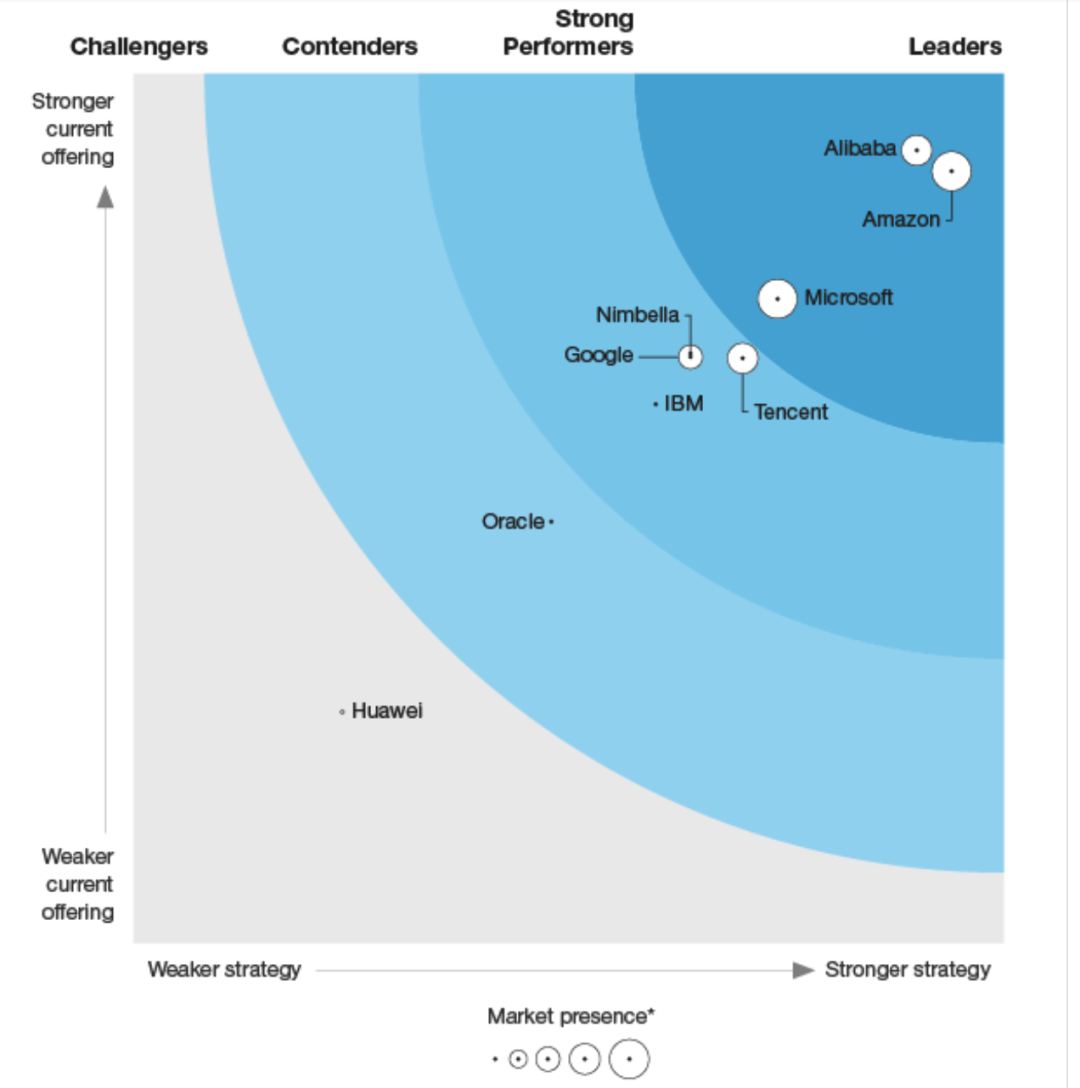
\includegraphics[width=0.7\linewidth]{images/faas-2021-q1.png}
    \caption{《Forrester Wave™:函数即服务 (FaaS) 平台,2021 年第一季度》评估结果\cite{serverless_report_2021}}
    \label{faas_2021_q1_ranking}
\end{figure}

\subsection{Serverless技术实现的核心问题}

Serverless技术在实现上,
一方面需要解决Serverless理念自身的技术要求所带来的挑战,
另一方面,在落地实际业务时,
也会收到实际业务影响而带来一些其他的问题。
总结来看,在Serverless技术实现上,
需要解决的核心问题有:

\begin{itemize}
    \item \textbf{弹性伸缩}:弹性伸缩是Serverless的基础,如何能够响应近乎“无限”的请求、根据需要自动伸缩,是Serverless平台最核心的要素之一。它又可以拆解为两个子问题:基础架构和伸缩算法。
    \item \textbf{冷启动优化}:由于Serverless一般按照时长计费,且需要支持极度的伸缩,因此,决定其伸缩效率的关键因素是启动时间。如何降低启动时间是一个需要解决的问题,该问题一般又可以等价于冷启动优化问题。
    \item \textbf{高可用保障}:保障平台在突发流量增长时能够从容应对、容忍临时软硬件故障
    \item \textbf{应用部署}:
    \item \textbf{安全性}:FaaS需要运行用户代码,如何进行安全隔离、
        保证函数调用之间互不影响,是非常重要的问题
    \item \textbf{整合现有系统}:
\end{itemize}

\subsection{AWS Lambda的演进}
各个Serverless平台都是在不断完善和改进的,
AWS Lambda在Serverless领域耕耘最久、积累最丰富,
因此Lambda的功能、架构演进十分具有参考价值。
AWS Lambda从发布之初到现在也经历过许多变化,
包含新功能的支持、架构的调整等,
如\cref{lambda_involution}所示。

\begin{figure}[ht!]
    \centering
    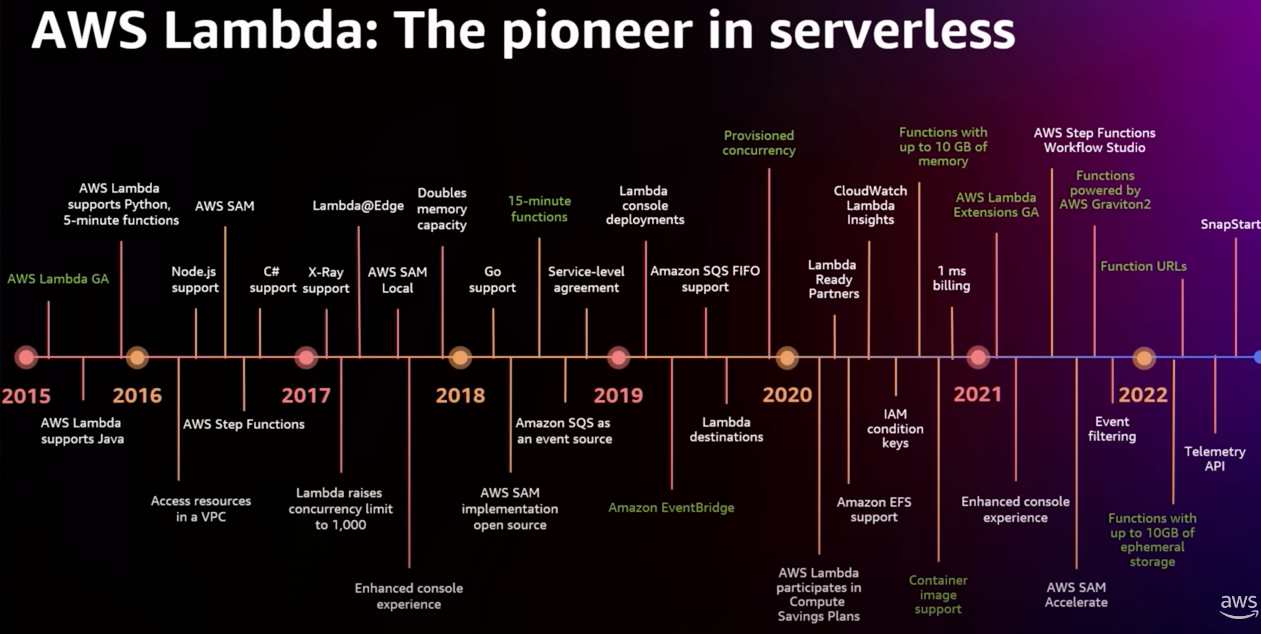
\includegraphics[width=\linewidth]{images/lambda_involution.png}
    \caption{AWS Lambda演进历史\cite{aws_lambda_2022}}
    \label{lambda_involution}
\end{figure}